This chapter presents the detailed engineering implementation of the Clothie fashion assistant framework, translating the proposed agentic architecture into a functional system. It documents the selection of the technology stack, the operational configuration of the core RAG components, the integration of multimodal search via FashionSigLIP, and the development of the mobile user interface.

The chapter is organized as follows: Section 4.1 outlines the project structure and pipeline organization, mapping every script in the repository to its functional responsibility. Section 4.2 details the development environment and the computational tech stack. Section 4.3 describes the implementation of the Orchestrator + Direct Routing backend using Gemini 2.5 Flash. Section 4.4 covers the integration of the Qdrant Vector Database and the optimization of the hybrid search pipeline. Section 4.5 illustrates the cross-platform mobile implementation using Flutter, and Section 4.6 presents the final system integration and deployment strategy.

\section{Project Structure and Pipeline Organization}
\label{sec:impl_structure}

Section~\ref{sec:impl_structure} maps every script and module that participates in either the offline data pipeline or the online serving pipeline back to a single repository tree. The codebase has two physical roots: \texttt{fashion\_agent/} hosts the Python backend (FastAPI app, agent, search engine, indexing, preprocessing); \texttt{clothie\_web/} hosts the Flutter web client. The two communicate exclusively across the HTTP and Server-Sent-Events surface documented in Section~\ref{sec:impl_ui}. Inside the backend root, files cluster into two functionally distinct pipelines: an \emph{offline} pipeline that prepares the knowledge base ahead of any user request, and an \emph{online} pipeline that handles each live conversation. Tables~\ref{tab:impl_offline_scripts}--\ref{tab:impl_frontend_files} catalogue the scripts in each pipeline and the responsibility of each.


\subsection{Pre-processing Pipeline}

The  pipeline is run once at deployment time --- and re-run only when the dataset, the captioning prompts, or the embedding model change --- to produce the Postgres tables and the Qdrant collection that the online pipeline reads. Table~\ref{tab:impl_offline_scripts} catalogues the four scripts that form this pipeline.

\begin{table}[H]
\centering
\caption{Offline pipeline scripts}
\label{tab:impl_offline_scripts}
\small
\begin{tabular}{p{6.0cm} p{8.6cm}}
\toprule
\textbf{Script} & \textbf{Responsibility} \\
\midrule
\texttt{processing\_data.py} & Kaggle dataset download, noise filtering (Algorithm~\ref{alg:data_filtering}), and Gemini-driven caption + dominant-color enrichment (Algorithm~\ref{alg:llm_enrichment}); writes \texttt{fashion\_items} and \texttt{fashion\_item\_enrichment} into Postgres. \\
\texttt{test\_processing\_data.py} & Smoke test on a one-row sample to validate API keys, Postgres schema, and Gemini output shape before the long batch run. \\
\texttt{indexing/build\_index.py} & Reads enriched rows from Postgres, encodes both image and text with Marqo-FashionSigLIP (Algorithm~\ref{alg:fashionsiglip}), composes the BM25 surface (Algorithm~\ref{alg:bm25_composition}), and upserts every point into the Qdrant \texttt{fashion\_products} collection (Algorithm~\ref{alg:build_index}). \\
\texttt{indexing/update\_text\_index.py} & Refreshes only the text vectors when captions change without re-encoding images; keeps the GPU pass off the critical path. \\
\bottomrule
\end{tabular}
\end{table}

\subsection{Online Backend Pipeline}

The online pipeline runs inside the \texttt{fashion-api} container on every chat turn. It is split across four packages: \texttt{agent/} (orchestration, intent classification, memory, prompts), \texttt{search/} (hybrid retrieval), \texttt{shared/} (LLM client abstraction), and \texttt{api/} (FastAPI / Gradio surfaces and analytics endpoints). Tables~\ref{tab:impl_online_agent_scripts} and~\ref{tab:impl_online_api_scripts} catalogue these.

\begin{table}[H]
\centering
\caption{Online agent (\texttt{fashion\_agent/agent/}, \texttt{search/}, \texttt{shared/}).}
\label{tab:impl_online_agent_scripts}
\small
\begin{tabular}{p{6.0cm} p{8.6cm}}
\toprule
\textbf{Script} & \textbf{Responsibility} \\
\midrule
\texttt{agent/fashion\_agent.py} & Top-level orchestrator: \texttt{chat()} and \texttt{chat\_stream()} drive the five-step direct-routing pipeline (Algorithm~\ref{alg:routing}); owns the four \texttt{TTLCache} slot stores. \\
\texttt{agent/intent\_classifier.py} & Single-call LLM intent classification with six-slot extraction (Algorithm~\ref{alg:intent_class}) under a strict JSON-shape contract. \\
\texttt{agent/slot\_completeness.py} & Per-session slot merge across turns (Algorithm~\ref{alg:ttlcache_memory}) and weighted ranked-slot readiness check (Algorithm~\ref{alg:slot_readiness}). \\
\texttt{agent/clarification\_gate.py} & Deterministic clarification-template selection from \texttt{COMBO\_TEMPLATES} (Algorithm~\ref{alg:build_clarification}); zero LLM calls when the gate fires. \\
\texttt{agent/memory.py} & Postgres connection pool, idempotent schema initialisation, sessions, conversation history, selections, soft preferences, and behaviour telemetry. \\
\texttt{agent/prompts.py} & Single source of truth for every prompt template and the multilingual \texttt{SLOT\_TEMPLATES} / \texttt{COMBO\_TEMPLATES} stores. \\
\texttt{agent/agentic\_orchestrator.py} & Scaffolding for Mode B / Mode C tool-calling orchestration; not on the live default code path. \\
\texttt{agent/tools.py} & Tool-schema definitions consumed by the agentic orchestrator. \\
\texttt{agent/utils.py} & Shared helpers: token accounting, language tagging, small string utilities. \\
\texttt{search/search\_engine.py} & Seven-stage PATH 1 hybrid search (Algorithm~\ref{alg:hybrid_search}): expansion $\rightarrow$ BM25 + image-vector + text-vector $\rightarrow$ RRF $\rightarrow$ RapidFuzz $\rightarrow$ BGE rerank $\rightarrow$ top-$k$. \\
\texttt{search/query\_expansion.py} & Short-query LLM expansion gate (Algorithm~\ref{alg:expand_query}); skipped on long queries. \\
\texttt{search/fusion.py} & Reciprocal-Rank-Fusion implementation (Equation~\ref{eq:rrf}, Algorithm~\ref{alg:rrf}). \\
\texttt{search/reranker.py} & BGE Reranker v2-m3 cross-encoder with the weighted blend ($0.7 \cdot \text{reranker} + 0.3 \cdot \text{RRF}$) of Algorithm~\ref{alg:rerank_blend}. \\
\texttt{search/image\_query\_engine.py} & PATH 2 image-bytes search (Algorithm~\ref{alg:path2_search}) and PNG validation (Algorithm~\ref{alg:validate_png}). \\
\texttt{shared/llm.py} & \texttt{LLMClient} Protocol exposing \texttt{generate()} and \texttt{stream()}; Gemini-only in production with stubs reserved for OpenAI / Anthropic backends. \\
\bottomrule
\end{tabular}
\end{table}

\begin{table}[H]
\centering
\caption{Online API surface (\texttt{fashion\_agent/api/}).}
\label{tab:impl_online_api_scripts}
\small
\begin{tabular}{p{6.0cm} p{8.6cm}}
\toprule
\textbf{Script} & \textbf{Responsibility} \\
\midrule
\texttt{api/main.py} & FastAPI app definition, lifespan hook (\texttt{init\_memory\_tables}), every chat / sessions / products / images / PATH 2 / analytics route, and the Gradio fallback panel mounted at \texttt{/}. \\
\texttt{api/analytics.py} & Thesis-evaluation endpoints: token-cost rollup, retrieval-accuracy aggregate, gender-A/B comparison; gated by the \texttt{X-Admin-Key} header. \\
\bottomrule
\end{tabular}
\end{table}

\subsection{Frontend Pipeline}

The Flutter web client is compiled once and served as static assets from a small Nginx container on port 3000. Inside \texttt{clothie\_web/lib/}, files are split by responsibility into transport, screens, widgets, models, routing, and theming. Table~\ref{tab:impl_frontend_files} catalogues the top-level entries.

\begin{table}[H]
\centering
\caption{Frontend pipeline files (\texttt{clothie\_web/lib/}).}
\label{tab:impl_frontend_files}
\small
\begin{tabular}{p{6.0cm} p{8.6cm}}
\toprule
\textbf{Path} & \textbf{Responsibility} \\
\midrule
\texttt{lib/main.dart} & Flutter application entry; wires the global theme provider and the declarative router. \\
\texttt{lib/services/api\_service.dart} & Single HTTP and SSE transport shim; manual SSE parser for POST streaming, since Flutter Web has no native \texttt{EventSource} for POST. \\
\texttt{lib/screens/} & Top-level routes: splash, register (demographics), chat, rating, and the \texttt{X-Admin-Key}-gated professor dashboard. \\
\texttt{lib/widgets/} & Re-usable UI components: \texttt{chat\_bubble}, \texttt{product\_card}, \texttt{thinking\_indicator}, \texttt{shimmer\_product\_grid}, \texttt{star\_rating}. \\
\texttt{lib/models/} & Typed DTOs for chat messages, products, cart items, and the professor-analytics rows. \\
\texttt{lib/router/} & Declarative route table consumed by \texttt{main.dart}. \\
\texttt{lib/extension/} & Build-time configuration (\texttt{kApiBaseUrl}) and theme-provider extensions. \\
\texttt{lib/theme/} & Centralised colour palette and \texttt{ThemeData} factory. \\
\bottomrule
\end{tabular}
\end{table}


\section{Technical Stack and Environment}
\label{sec:impl_stack}

\textbf{Technical Stack and Environment} catalogues the runtime artefacts that turn the algorithms of \textbf{Methodology} into a deployed service. Whereas Methodology argues \emph{why} the system processes a query in a given way, this section answers \emph{which versions, on which devices, in which directories, and under which environment variables} those algorithms actually execute. The chapter therefore avoids restating any algorithmic claim already labelled in Methodology; instead, it cross-references the relevant labels (e.g.\ \textbf{Hybrid Search}, \textbf{Direct Routing}) and concentrates on engineering specifics.


\subsection{Component Inventory}

The Clothie reference deployment is a single Docker Compose stack on a 16\,GB Apple-Silicon workstation. Table~\ref{tab:impl_stack_components} enumerates every component in production use, its pinned version (or version constraint as expressed in \texttt{requirements-docker.txt} and \texttt{docker-compose.yml}), and its functional role.

\begin{table}[H]
\centering
\caption{Runtime components in the Clothie deployment.}
\label{tab:impl_stack_components}
\footnotesize
\begin{tabular}{>{\raggedright\arraybackslash}p{4.0cm} >{\raggedright\arraybackslash}p{3.0cm} >{\raggedright\arraybackslash}p{7.0cm}}
\toprule
\textbf{Component} & \textbf{Version / image} & \textbf{Role} \\
\midrule
Python runtime & 3.11-slim & Hosts the FastAPI process, the agent, the search engine, and the model loaders. \\
FastAPI & $\geq 0.104$ & HTTP server exposing \texttt{/api/chat}, \texttt{/api/chat/stream}, sessions, products, images, and analytics. \\
Uvicorn \texttt{[standard]} & $\geq 0.24$ & ASGI worker driving FastAPI under the same process as Gradio. \\
Gradio & $\geq 4.0$ & Fallback chat UI mounted at \texttt{/} for development sanity checks. \\
Pydantic & $\geq 2.0$ & Request / response validation for every API route. \\
PostgreSQL & \texttt{postgres:}\newline\texttt{16-alpine} & Source of truth for sessions, conversation history, selections, ratings, token usage, impressions, clicks, intents, orders. \\
Qdrant & \texttt{qdrant/}\newline\texttt{qdrant:latest} & Vector store for image and text embeddings; collection \texttt{fashion\_products}. \\
\texttt{psycopg2-binary} & $\geq 2.9.9$ & Sole Postgres driver; used through a module-level \texttt{SimpleConnectionPool}. \\
\texttt{qdrant-client} & $\geq 1.7$ & HTTP client to Qdrant, prefer-gRPC disabled for local container reach. \\
\texttt{rank-bm25} & $\geq 0.2.2$ & In-memory BM25 lexical retriever rebuilt on API startup (Algorithm~\ref{alg:bm25_composition}). \\
\texttt{rapidfuzz} & $\geq 3.5$ & Soft post-fusion filter on tokenised captions / labels. \\
\texttt{open-clip-torch}\newline + Marqo-FashionSigLIP & $\geq 2.24$ / 768-d & Cross-modal encoder used by Algorithm~\ref{alg:fashionsiglip} to project images and queries into a shared cosine space. \\
\texttt{transformers}\newline + BGE Reranker v2-m3 & $\geq 4.36$ & Cross-encoder used by Algorithm~\ref{alg:rerank_blend} to score the fused candidate set. \\
\texttt{torch} & $\geq 2.1$ & Tensor backend for both encoders; chooses the device at first use. \\
Gemini 2.5 Flash\newline(\texttt{google-generativeai}) & $\geq 0.3$ & The single LLM client wired into intent classification (Algorithm~\ref{alg:intent_class}), query expansion (Algorithm~\ref{alg:expand_query}), and synthesis (Algorithm~\ref{alg:synthesize_response}). \\
Flutter (web) & 3.x stable & Cross-platform shell compiled to JS, served from a Nginx container on port 3000. \\
Docker Compose & v2 plugin & Orchestrates the five services described in Section~\ref{sec:impl_deploy}. \\
ngrok agent & \texttt{ngrok/ngrok:}\newline\texttt{latest} & Public-URL tunnel; binds a reserved \texttt{*.ngrok-free.app} subdomain to \texttt{clothie-web:80}. \\
\bottomrule
\end{tabular}
\end{table}

The repository keeps two requirements files: \texttt{requirements-docker.txt} pins the runtime libraries above, while \texttt{requirements-dev.txt} adds Jupyter and pandas for offline notebooks under \texttt{analysis/}. The container image installs only the former, keeping the production footprint smaller than the developer footprint.

\subsection{Hardware and Model-Loading Strategy}

The reference platform is a 16\,GB Apple-Silicon laptop. The agent selects its torch device at first model use: if \texttt{torch.backends.mps.is\_available()} returns true, embeddings and reranking run on the Metal-Performance-Shaders backend; otherwise the agent falls back to CPU. The selected device is logged once during the cold-start of \texttt{api.main:lifespan}; subsequent encode/score calls reuse it.

The two models that dominate the on-disk footprint are cached under the directory bound to the \texttt{HF\_HOME} environment variable (set to \texttt{/app/models} in the container). Marqo-FashionSigLIP weighs approximately 1\,GB (768-dimensional ViT backbone plus tokenizer); BGE Reranker v2-m3 weighs approximately 1\,GB (XLM-RoBERTa large with cross-encoder head). On a fresh machine the first \texttt{docker compose up} pulls roughly 3.7\,GB of HuggingFace artefacts into the cache; subsequent restarts read from disk and complete in under a minute. The two singletons (\texttt{FashionEmbedder}, \texttt{BGEReranker}) are constructed lazily at first use and cached in module-level globals so that all subsequent requests share one weight copy per process.

\subsection{Repository Layout}

The deployable artefacts are organised across three sibling directories under the repository root, plus a one-command launcher:

\begin{itemize}[leftmargin=1.5em,itemsep=2pt,topsep=2pt]
    \item \texttt{fashion\_agent/} --- the Python backend: FastAPI routes (\texttt{api/}), the orchestrator (\texttt{agent/}), the seven-stage hybrid search engine (\texttt{search/}), the offline ingestion / indexing pipelines (\texttt{pre\_processing/}, \texttt{indexing/}), and the OpenSpec change-log mirror under \texttt{openspec/}. The \texttt{Dockerfile}, \texttt{docker-compose.yml}, and the two requirements files live at this level.
    \item \texttt{clothie\_web/} --- the Flutter codebase compiled to web. The single transport shim is \texttt{lib/services/api\_service.dart}; the screen- and widget-level state is split across \texttt{lib/screens/} and \texttt{lib/widgets/}. Built artefacts are served on port 3000 from a small Nginx container.
    \item \texttt{qwen\_local\_rag/} --- a frozen, pre-thesis local-RAG experiment retained for archival reference; not invoked by any production code path.
    \item \texttt{start.sh} (repo root) --- the one-command launcher that resolves Docker on macOS, brings up the databases, waits for healthchecks, builds and runs the application services, and prints the public tunnel URL once the front-end is reachable.
\end{itemize}


\section{Agentic Reasoning and Prompt Engineering}
\label{sec:impl_prompts}

Section~\ref{sec:impl_prompts} documents the prompt artefacts that drive intent classification, slot extraction, query expansion, and answer synthesis, together with their parse-time contract and fallback behaviour. The algorithmic flow is already specified in Methodology --- Algorithm~\ref{alg:intent_class} for the LLM-based classifier with six-slot extraction, Algorithm~\ref{alg:slot_readiness} for the deterministic readiness gate, Algorithm~\ref{alg:resolve_search_query} for the query that finally enters retrieval, and Algorithm~\ref{alg:synthesize_response} for the closing synthesis step --- so the implementation chapter restricts itself to artefact identity, expected JSON shape, and what the system does when an LLM call drifts off contract.

\subsection{Prompt Artefact Inventory}

Every prompt template lives in a single Python module (\texttt{agent/prompts.py}); inlining prompts elsewhere is forbidden by an in-file warning so that every template remains reviewable in one place. The body of the central template, \texttt{INTENT\_PROMPT}, is reproduced verbatim below; Table~\ref{tab:impl_prompt_artefacts} then catalogues every prompt artefact and its parse contract.

\begin{table}[H]
\centering
\caption{Prompt artefacts in \texttt{agent/prompts.py} and their parse contract.}
\label{tab:impl_prompt_artefacts}
\scriptsize
\begin{tabular}{p{4.0cm} p{6.0cm} p{4.2cm}}
\toprule
\textbf{Name} & \textbf{Purpose / expected JSON shape} & \textbf{Fallback on parse failure} \\
\midrule
\texttt{INTENT\_PROMPT} & Single-call intent classification, six-slot extraction, and selection-number extraction. JSON: \texttt{intent}, \texttt{confidence}, \texttt{filters}, \texttt{refined\_query}, six \texttt{slot\_*}, \texttt{selected\_numbers}. & Treat as \texttt{unclear}; route to the deterministic clarification gate (Algorithm~\ref{alg:build_clarification}). \\
\texttt{SYNTHESIS\_PROMPT} & Non-streamed final answer with optional styling tip; locked to the detected language. JSON: \texttt{answer}, \texttt{styling\_suggestion}. & Use raw text as \texttt{answer}; leave \texttt{styling\_suggestion} empty. \\
\texttt{STREAM\_SYNTHESIS\_\allowbreak PROMPT} & Streaming variant; emits plain text and an inline ``Styling tip:'' marker rather than JSON. & Plain text already; no recovery needed. \\
\texttt{EXPANSION\_PROMPT} & Short paraphrases of the user query for BM25 recall (Algorithm~\ref{alg:expand_query}); returns a JSON array of strings. & Use only the original query; skip expansion. \\
\texttt{CLARIFICATION\_\allowbreak PROMPT} & LLM-driven clarification used only when the deterministic gate cannot construct one. JSON: \texttt{question}. & Use the per-language \texttt{FALLBACK\_QUESTION}. \\
\texttt{OUT\_OF\_SCOPE\_\allowbreak RESPONSE}, \texttt{UNSUPPORTED\_\allowbreak CATEGORY\_RESPONSE} & Static refusal / redirect strings keyed by language; not LLM calls. & --- \\
\bottomrule
\end{tabular}
\end{table}

Every JSON-bearing template ends with the literal instruction \emph{Respond with ONLY a JSON object}. The orchestrator nonetheless treats this as advice rather than guarantee: every parse path validates the response, and on failure routes through the deterministic fallback recorded in the rightmost column.

\subsection{Multilingual Templates}

The deterministic clarification gate of Algorithm~\ref{alg:build_clarification} relies on two template stores keyed by language and by missing-slot configuration. The first, \texttt{SLOT\_TEMPLATES}, maps each individual slot (\texttt{category}, \texttt{color}, \texttt{fabric}, \texttt{fit}) to a one-line example phrasing in English (\texttt{en}), Vietnamese (\texttt{vi}), and Spanish (\texttt{es}). The second, \texttt{COMBO\_TEMPLATES}, is keyed by a \texttt{frozenset} of missing slots: \texttt{\{category,color\}}, \texttt{\{color,fabric,fit\}}, \texttt{\{fabric,fit\}}, \texttt{\{color\}}, \texttt{\{category\}}, and the four-slot combination \texttt{\{category,color,fabric,fit\}}, each with all three language variants. The gate first looks up the combination; if none matches, it concatenates per-slot lines from \texttt{SLOT\_TEMPLATES}. Because the lookup is total over the supported missing-slot configurations, the deterministic branch never falls through to an LLM call --- this is the empirical basis for the ``zero LLM calls when the gate fires'' claim made in Methodology Section~\ref{sec:gating}.

Language detection itself is purely lexical: the helper \texttt{detect\_language(text)} matches Vietnamese diacritics first (since the Vietnamese tonal alphabet has no Spanish overlap), then unambiguous Spanish tokens (\texttt{ñ}, \texttt{¿}, \texttt{¡}, plus a curated whitelist of Spanish-only words), then defaults to English. The decision flows through into both clarification rendering and the synthesis prompt's \texttt{language} field, ensuring the answer is rendered in the user's language without a separate translation call.

\subsection{Synthesis and Streaming}

Synthesis has two siblings sharing a base body. \texttt{SYNTHESIS\_PROMPT} requests a strict JSON object with two fields, \texttt{answer} and \texttt{styling\_suggestion}; this path is invoked by the non-streaming chat endpoint. \texttt{STREAM\_SYNTHESIS\_PROMPT} appends a single instruction --- \emph{Respond with plain text only (NO JSON format)} --- so that the SSE channel can yield token-level chunks directly to the client without a closing parse step. Both prompts hard-bind the response language, forbid claims about ``cart'' or ``checkout'' (Clothie is a research surface, not a transactional one), and end with a fixed call-to-action string per intent. Two further variants (\texttt{SYNTHESIS\_PROMPT\_AGENTIC} and its streaming companion) exist for the experimental Mode~B / Mode~C tool-calling orchestrators; the live default is the direct route, so those variants are scaffolding and are not exercised in production.

\subsection{Failure Modes}

The orchestrator is engineered to keep a session alive even when an LLM call misbehaves. Three failure classes recur and are each handled deterministically.

\begin{itemize}[leftmargin=1.5em,itemsep=2pt,topsep=2pt]
    \item \emph{Malformed JSON from intent classification.} The orchestrator catches \texttt{JSONDecodeError}, treats the call as if intent had been \texttt{unclear} with confidence zero, and routes to the deterministic clarification gate. No retry is attempted; the user simply sees a clarification question instead of a search.
    \item \emph{Low-confidence drift.} Even with a parseable response, the readiness check of Algorithm~\ref{alg:slot_readiness} requires a weighted four-slot score above \texttt{SEARCH\_CONFIDENCE\_THRESHOLD} (default 0.75). When the threshold is not crossed, the gate fires and no retrieval is launched.
    \item \emph{Unsupported category.} If the classified \texttt{slot\_category} sits outside the catalogue's coarse taxonomy, the orchestrator emits a per-language \texttt{UNSUPPORTED\_CATEGORY\_RESPONSE} via the \texttt{clarification} SSE event and yields a \texttt{done} event with intent \texttt{unsupported\_category}; no Qdrant call is made, and no token budget is spent on a doomed retrieval.
\end{itemize}


\section{Knowledge Base and Vector Indexing}
\label{sec:impl_kb}

Section~\ref{sec:impl_kb} documents how the knowledge base of Chapter~\ref{chap:methodology} is laid out on disk and across containers in the running deployment. Algorithm~\ref{alg:build_index} formalises the index-building pipeline; Algorithm~\ref{alg:fashionsiglip} formalises the cross-modal encoding step that produces the vectors stored here; this section restricts itself to deployment specifics that examiners cannot reproduce without seeing the running system.

\subsection{Qdrant Collection as Deployed}

The Qdrant container exposes port 6333 on the internal Compose network and is reached by the API container at \texttt{http://qdrant:6333}. There is exactly one collection in use, \texttt{fashion\_products}, configured with two named vectors --- \texttt{image\_vector} and \texttt{text\_vector} --- both 768-dimensional and both using cosine distance. Each point's payload carries six fields: \texttt{image\_id} (the stable identifier shared with Postgres), \texttt{label} (the coarse class label from the Kaggle dataset), \texttt{color} (the dominant-color tag derived during enrichment), \texttt{caption} (the LLM-authored multimodal caption), \texttt{image\_path} (the host-side filename used by the image-serving endpoint), and \texttt{bm25\_content} (the tokenised lexical surface used to rebuild BM25 in memory). Every payload field has a single concrete value per point; there are no nested arrays, which keeps the in-process BM25 rebuild a simple iteration.

The BM25 retriever is intentionally not persisted to disk. On every API process start, the lifespan hook iterates the Qdrant points, reads \texttt{bm25\_content} from each payload, and constructs a fresh \texttt{rank\_bm25.BM25Okapi} instance keyed by index in iteration order. This design guarantees BM25 freshness without a migration step: any payload edit applied to Qdrant becomes lexically searchable on the next API restart, and there is no on-disk index file to drift away from the vector store.

\subsection{Postgres Schema and Connection Pooling}

Postgres exposes port 5432 on the internal network and is initialised on first startup by \texttt{init\_memory\_tables} in \texttt{agent/memory.py}. The function is idempotent: every \texttt{CREATE TABLE} uses \texttt{IF NOT EXISTS} and every column addition is gated on \texttt{ADD COLUMN IF NOT EXISTS}. New deployments therefore receive the full schema on first run; existing deployments receive only the missing pieces. Table~\ref{tab:impl_pg_tables} summarises the relations actually created.

\begin{table}[H] \centering \caption{Postgres relations initialised at API startup.} 
  \label{tab:impl_pg_tables} \small \begin{tabular}{p{4.4cm} p{3.0cm} p{6.6cm}} \toprule 
  \textbf{Relation} & \textbf{Primary key} & \textbf{Role} \\ \midrule \texttt{user\_sessions} & 
  \texttt{session\_id} & Stores session profile, demographic fields, preferred model, and JSONB 
  preference history. \\ \texttt{conversation\_history} & \texttt{id} (BIGSERIAL) & Stores the ordered 
  user--assistant message history for each session. \\ \texttt{selected\_items} & \texttt{id} & Records 
  products explicitly selected by the user from recent recommendations. \\ \texttt{user\_ratings} & 
  \texttt{id} & Stores post-session ratings and optional free-text feedback. \\ 
  \texttt{llm\_token\_usage} & \texttt{id} & Logs per-call token usage by model and call type for cost 
  analysis. \\ \texttt{product\_impressions}, \texttt{product\_clicks}, \texttt{product\_intents} & 
  \texttt{id} & Tracks product exposure, clicks, and intent events for engagement analysis. \\ 
  \texttt{user\_orders} & \texttt{id} & Stores simulated checkout records and marks the session as 
  completed. \\ \texttt{cart\_removals} & \texttt{id} & Records product removals from the cart for 
  removal-rate analysis. \\ \bottomrule \end{tabular} \end{table}

Connection management is handled by a module-level \texttt{SimpleConnectionPool} configured with \texttt{minconn=2}, \texttt{maxconn=10}, \texttt{connect\_timeout=5}, and a server-side \texttt{lock\_timeout} of 8\,s applied through \texttt{options}. A lightweight \texttt{\_db\_conn()} context manager borrows and returns a connection per logical operation, keeping all explicit \texttt{conn.close()} calls out of the request handlers. Two soft-preference columns on \texttt{user\_sessions} --- \texttt{liked\_items} and \texttt{query\_history} --- use the JSONB type with default \texttt{[]}; this is what allows ~\texttt{add\_liked\_item} and ~\texttt{log\_query\_history} to be implemented as single \texttt{UPDATE} statements with \texttt{jsonb} concatenation.

\subsection{Model Cache Layout}

Both the SigLIP encoder and the BGE reranker resolve their weights through HuggingFace Hub. The \texttt{HF\_HOME} environment variable (set to \texttt{/app/models} in the API container, bound to a host-side \texttt{./models/} directory) directs the library to a single cache root. Inside that directory HuggingFace creates the canonical sub-tree --- \texttt{hub/models--Marqo--marqo-fashionsiglip/...} for the encoder and \texttt{hub/models--BAAI--bge-reranker-v2-m3/...} for the reranker --- so deletion or replacement of a model is a directory operation rather than a code change. On a cold start with no cache, the first encoded query triggers a download of approximately 3.7\,GB; subsequent starts complete in seconds. The deployment recommendation is therefore to pre-warm the host \texttt{./models/} directory before exposing the public URL.

\subsection{Volume Lifecycle and Backup}

The \texttt{docker-compose.yml} declares two named volumes: \texttt{pgdata} for Postgres data and \texttt{qdrant\_data} for the Qdrant collection. Both are persistent across \texttt{docker compose down}; both are deleted by \texttt{docker compose down -v}. The handover document distinguishes safe and destructive shutdown explicitly, because deleting either volume forces the multi-hour re-ingestion pipeline (Kaggle download $\rightarrow$ Algorithm~\ref{alg:data_filtering} $\rightarrow$ Algorithm~\ref{alg:llm_enrichment} $\rightarrow$ Algorithm~\ref{alg:build_index}) to run again.

To make transfer between machines tractable, the repository ships two on-disk archives: \texttt{pgdata\_backup.tar.gz} (approximately 69\,MB) and \texttt{qdrant\_backup.tar.gz} (approximately 59\,MB). Restoration creates the two named volumes (\texttt{fashion\_agent\_pgdata} and \texttt{fashion\_agent\_qdrant\_data}), launches a transient Alpine container that mounts the volume and the host backup directory, and extracts the archive into the volume. The procedure does not require Postgres or Qdrant to be running, and it runs in well under a minute on a local SSD; the alternative path of re-ingesting from Kaggle takes hours and incurs roughly thirty thousand Gemini calls for caption / color enrichment, so the archive route is the recommended onboarding flow.


\section{Multimodal Interface Development}
\label{sec:impl_ui}

The user-facing surfaces are split across two clients --- a Flutter web application that ships to end users and a Gradio chat panel mounted at the FastAPI root for development sanity checks --- talking to the same FastAPI backend. Both clients consume the same Server-Sent-Events (SSE) channel, so the same chat behaviour is exercisable from a polished cross-platform shell or from a one-page debugging surface without rebuilding the API.

\subsection{Gradio Fallback UI}

The Gradio panel at \texttt{http://localhost:8000/} is built from \texttt{api/main.py:create\_gradio\_app}. It binds a single text input, a chat panel, and a per-session state field; on submit it iterates \texttt{agent\_chat\_stream} and parses each SSE event with a small in-process helper, accumulating tokens into the chat bubble, formatting product data into a markdown product list with embedded \texttt{/api/images/<filename>} URLs, and rendering thinking events inside an HTML \texttt{<details>} block. The panel exists primarily as a diagnostic surface --- an examiner can replicate any user-visible behaviour without touching the Flutter build pipeline --- and as a fallback if the Flutter container is unavailable.

\begin{figure}[H]
    \centering
    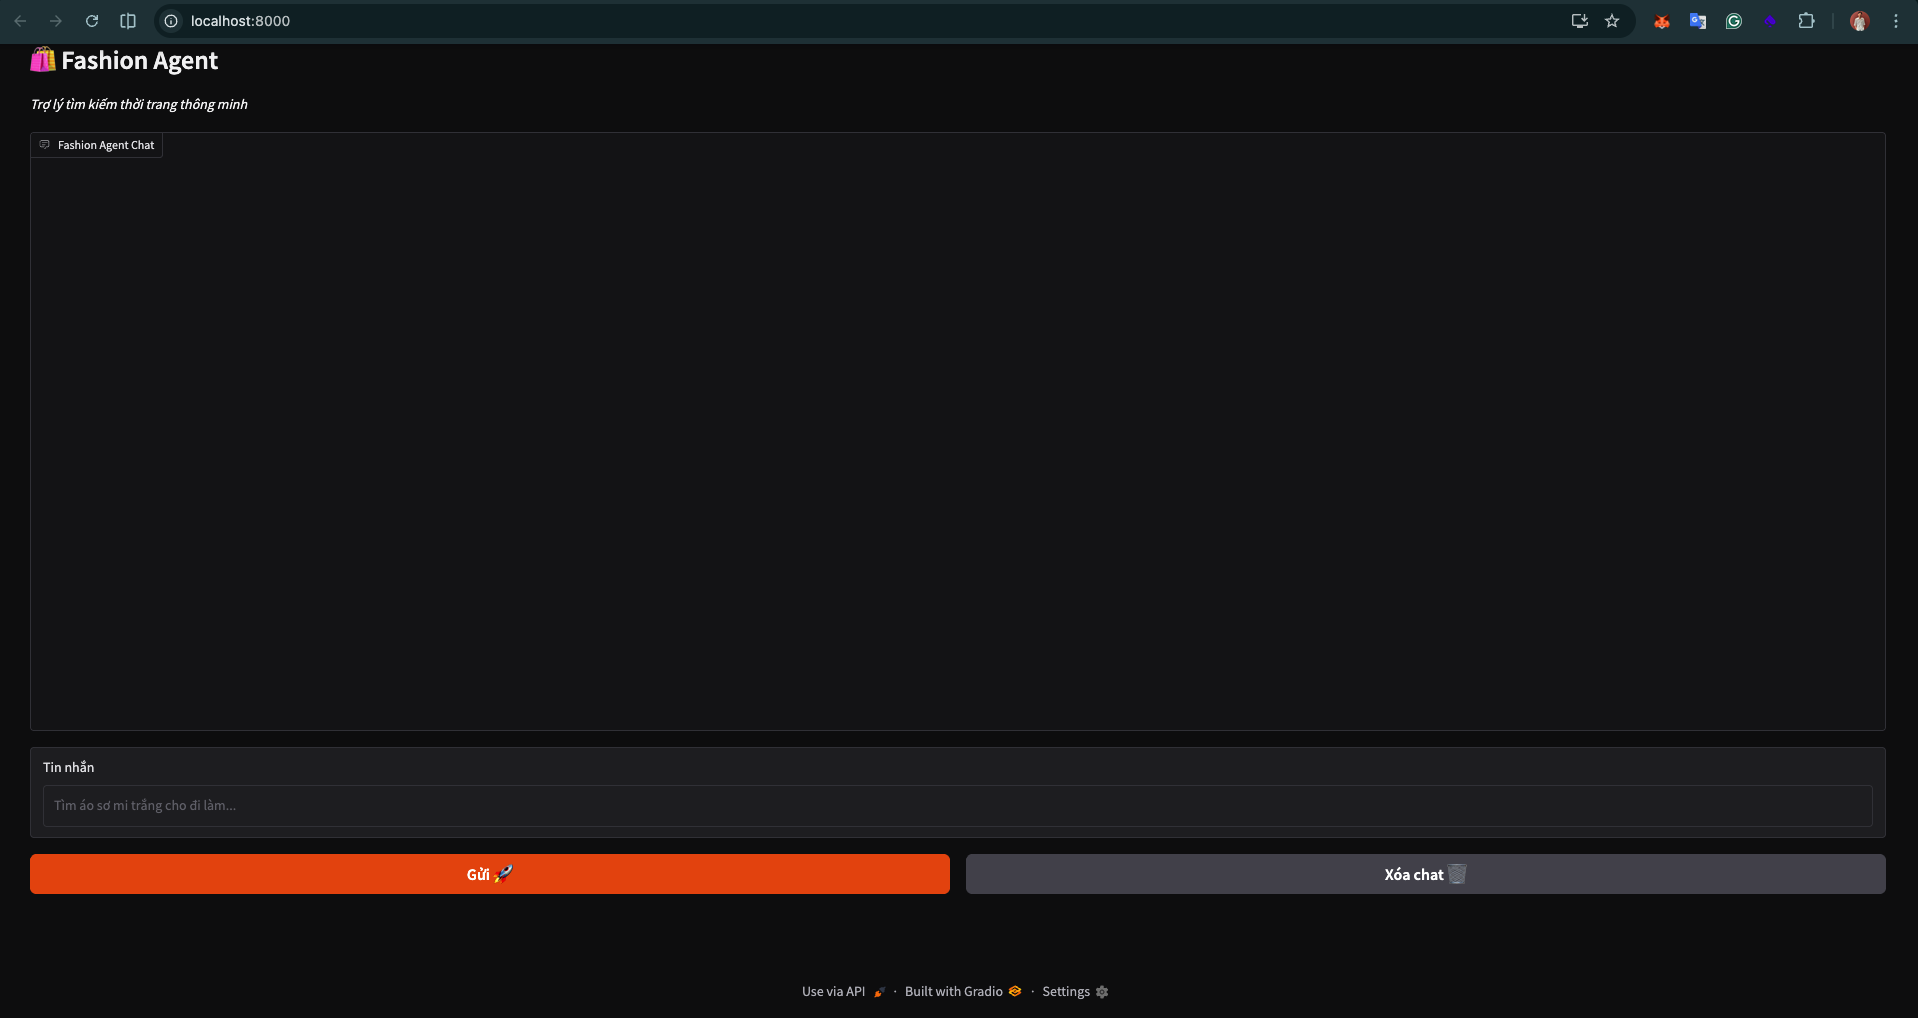
\includegraphics[width=0.85\textwidth]{screenshot_path1_clarification.png}
    \caption{PATH 1 multi-turn flow in the Gradio fallback UI: the deterministic clarification gate fires after the user enters an underspecified query, the user replies with the missing slots, and the resulting hybrid-search gallery renders with thinking events visible inside the collapsible block.}
    \label{fig:impl_path1_clarification}
\end{figure}

\subsection{Flutter Web Client}

The Flutter shell under \texttt{clothie\_web/} compiles to JavaScript and is served from a small Nginx container on port 3000; it is the surface every end user actually meets. The transport layer is a single file --- \texttt{lib/services/api\_service.dart} --- which exposes typed methods for session creation, the chat SSE stream, cart fetch, ratings, demographics, and behaviour analytics. Because Flutter Web cannot use a native \texttt{EventSource} for POST, the SSE consumer is implemented manually: \texttt{ApiService.chatStream} sends a \texttt{POST} \texttt{/api/chat/stream}, line-splits the response stream, accumulates an event-name and a data line, and yields a typed \texttt{SseEvent} on every blank-line boundary.

The application's screen graph is small and intentional. The main chat screen renders \texttt{ChatBubble}, \texttt{ProductCard}, and \texttt{ShimmerProductGrid} widgets driven by the SSE stream above; the \texttt{rating} screen submits a 1--5 triple plus free-text feedback at end-of-session; and the \texttt{professor\_dashboard} screen consumes the analytics endpoints behind the \texttt{X-Admin-Key} header. The reasoning indicator is rendered by the \texttt{thinking\_indicator} widget so that the SSE \texttt{thinking\_*} sub-protocol drives a single visual element.

\begin{figure}[H]
    \centering
    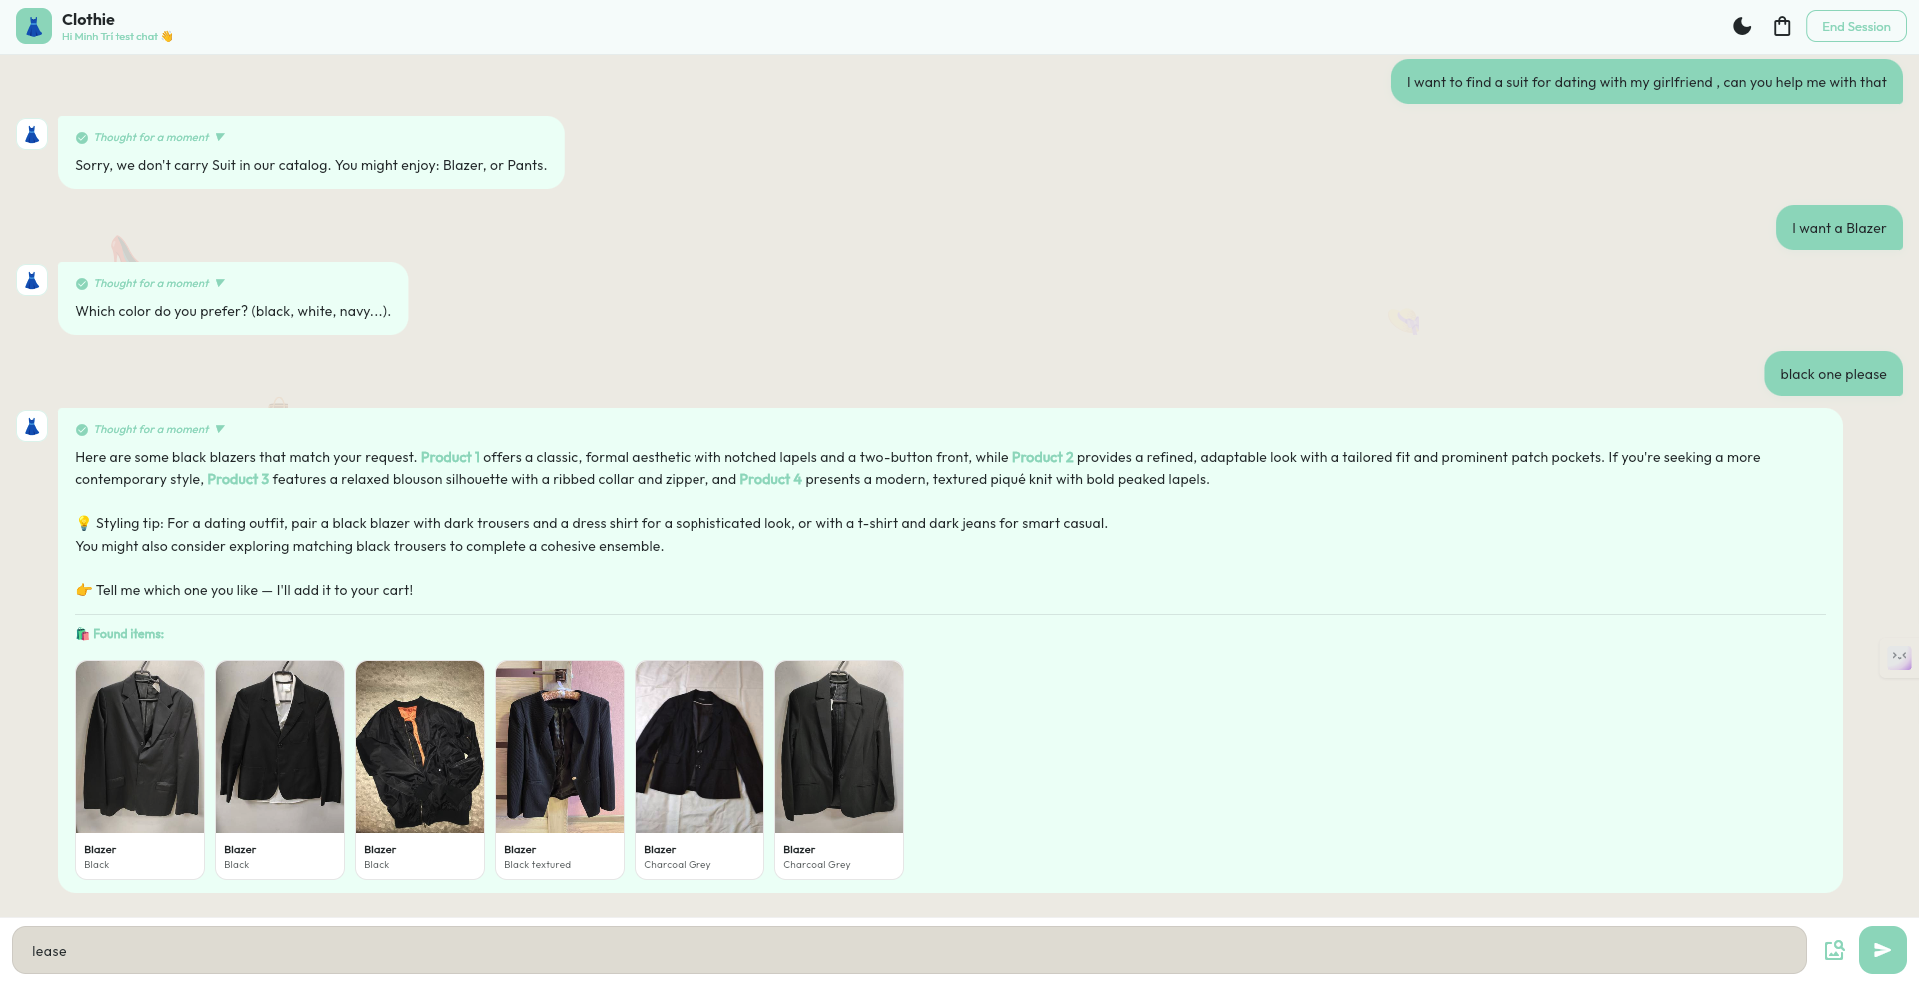
\includegraphics[width=0.85\textwidth]{screenshot_path1_multilingual.png}
    \caption{Text-to-image in the Flutter web client.}
    \label{fig:impl_path1_multilingual}
\end{figure}

\begin{figure}[H]
    \centering
    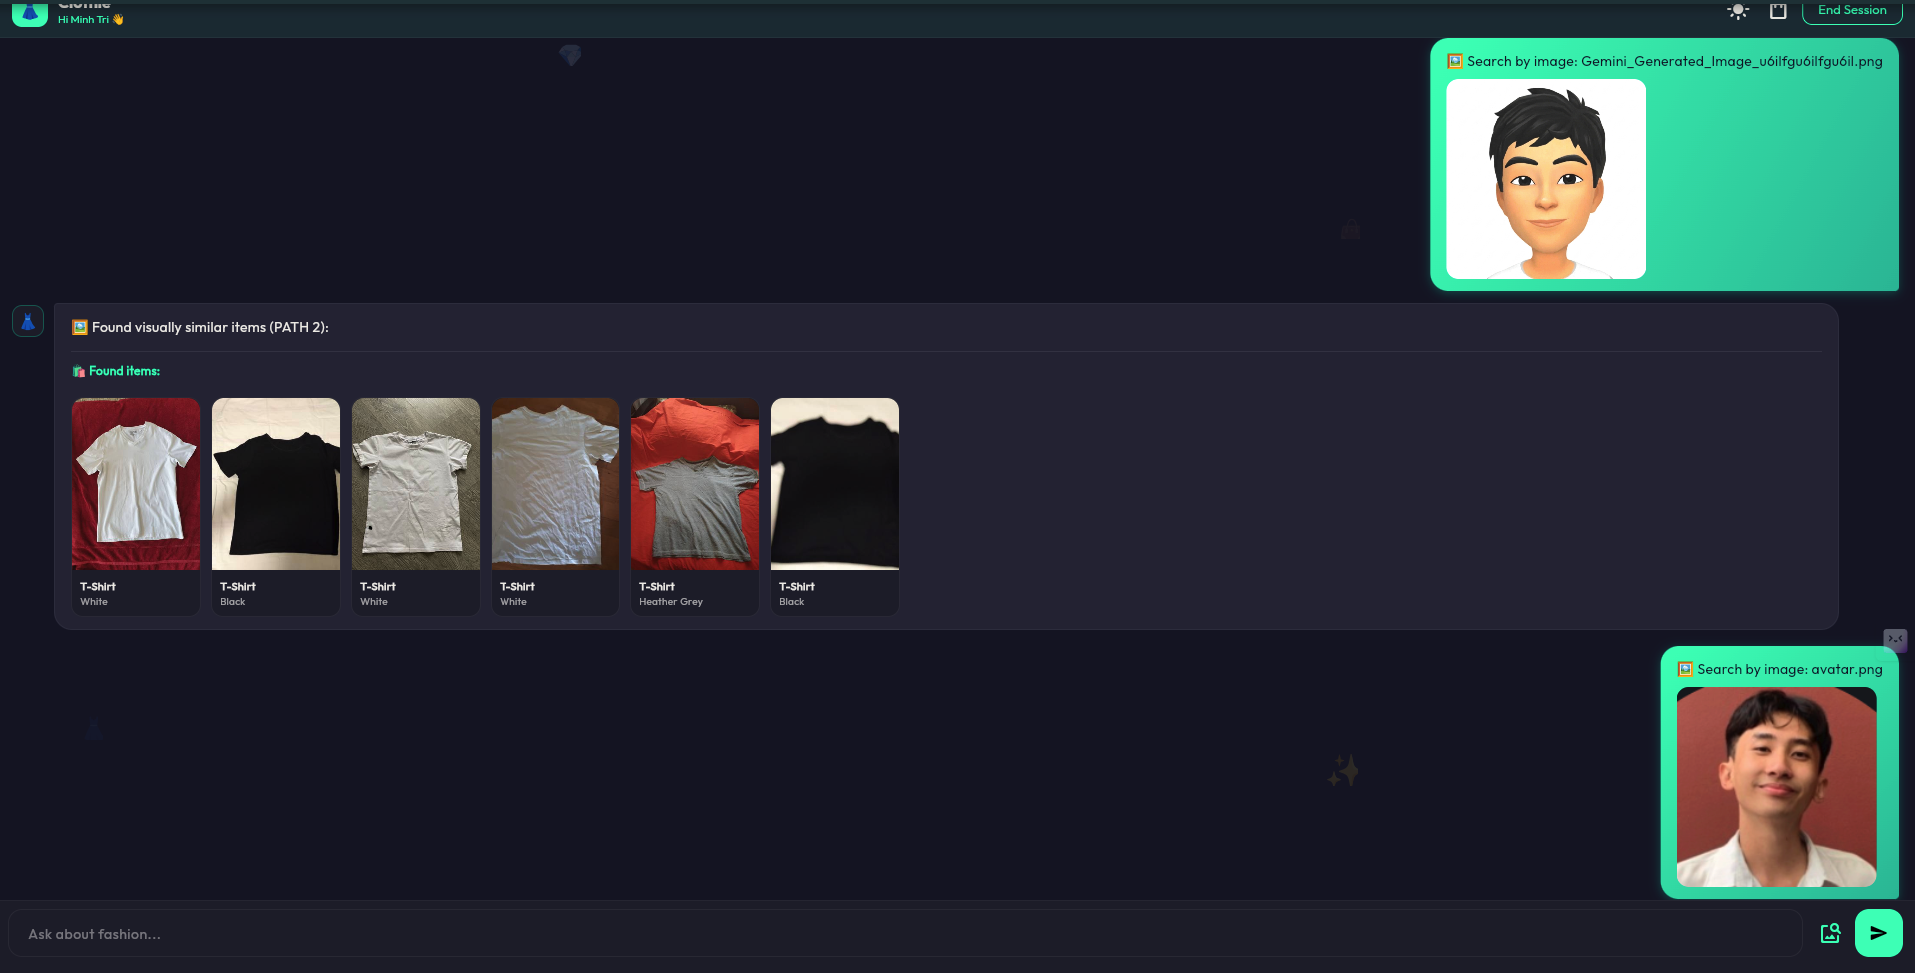
\includegraphics[width=0.85\textwidth]{screenshot_path2_image_search.png}
    \caption{PATH 2 image-to-image search: the user uploads a PNG via the image-attach widget.}
    \label{fig:impl_path2_image_search}
\end{figure}

The Flutter--FastAPI contract is small and stable. Table~\ref{tab:impl_endpoints} enumerates the endpoints actually consumed by \texttt{api\_service.dart} and the Gradio panel.

\begin{table}[H]
\centering
\caption{API endpoints consumed by the front-ends.}
\label{tab:impl_endpoints}
\footnotesize
\setlength{\tabcolsep}{4pt}
\begin{tabular}{>{\raggedright\arraybackslash\ttfamily}p{4.6cm} >{\raggedright\arraybackslash}p{1.6cm} >{\raggedright\arraybackslash}p{4.0cm} >{\raggedright\arraybackslash}p{4.0cm}}
\toprule
\textbf{\normalfont Path} & \textbf{Method} & \textbf{Request} & \textbf{Response} \\
\midrule
/api/sessions & POST & \texttt{user\_name}, \texttt{year\_of\_birth}, \texttt{gender}, \texttt{preferred\_model} & \texttt{session\_id} \\
/api/chat & POST & \texttt{message}, \texttt{session\_id} & Non-streamed answer + product list. \\
/api/chat/stream & POST & \texttt{message}, \texttt{session\_id} & SSE stream (Table~\ref{tab:impl_sse}). \\
/api/products/\{image\_\allowbreak id\} & GET & --- & Product row joined with enrichment. \\
/api/images/\{filename\} & GET & --- & PNG / JPEG static file. \\
/api/path2/image-search & POST & \texttt{image} (PNG), \texttt{session\_id}, \texttt{top\_k} & Visually-similar product list. \\
/api/sessions/\{sid\}/\allowbreak selections & GET /\newline POST /\newline DELETE & --- / \texttt{image\_id}, \texttt{label}, \texttt{color}, \texttt{caption}, \texttt{image\_path}, \texttt{position}, \texttt{path\_mode} & Cart contents / insert ack / removal ack. \\
/api/sessions/\{sid\}/\allowbreak impressions & POST & list of \texttt{image\_id}, \texttt{position}, \texttt{search\_query}, \texttt{path\_mode} & Logged-count ack. \\
/api/sessions/\{sid\}/\allowbreak clicks & POST & \texttt{image\_id}, \texttt{position}, \texttt{search\_query}, \texttt{path\_mode} & Ack. \\
/api/sessions/\{sid\}/\allowbreak intents & POST & \texttt{image\_id}, \texttt{intent\_type} ($\in$\{\texttt{will\_buy}, \texttt{not\_for\_me}\}), \texttt{path\_mode} & Ack. \\
/api/sessions/\{sid\}/\allowbreak orders & POST & \texttt{phone}, \texttt{address}, \texttt{path\_mode} & \texttt{order\_id} (also stamps \texttt{ended\_at}). \\
/api/rating & POST & three 1--5 ratings + \texttt{feedback} & Ack. \\
/health & GET & --- & Postgres / Qdrant liveness probe. \\
\bottomrule
\end{tabular}
\end{table}

\subsection{Streaming Protocol (Server-Sent Events)}

The streaming endpoint \texttt{/api/chat/stream} is the production path; the non-streaming \texttt{/api/chat} is a thin wrapper that drains the same generator into a single response. Each event the orchestrator yields is encoded by the \texttt{\_sse(event, data)} helper into the standard SSE wire format (an \texttt{event:} line, a \texttt{data:} line carrying a JSON-encoded payload, and a blank line). Table~\ref{tab:impl_sse} enumerates every event type emitted by \texttt{chat\_stream()} together with the schema of its \texttt{data} field, cross-checked against the actual \texttt{\_sse(...)} call sites in \texttt{agent/fashion\_agent.py}.

\begin{table}[H]
\centering
\caption{SSE event types emitted by \texttt{chat\_stream()} and the schema of each \texttt{data} field.}
\label{tab:impl_sse}
\small
\begin{tabular}{p{3.2cm} p{8.4cm}}
\toprule
\textbf{Event} & \textbf{Data fields} \\
\midrule
\texttt{thinking\_start} & \texttt{text}: label of the first thinking step. \\
\texttt{thinking\_step} & \texttt{detail}: intermediate step (intent, slot merge, search). \\
\texttt{thinking\_end} & \texttt{duration\_ms}, \texttt{input\_tokens}, \texttt{output\_tokens}: timing and token counters. \\
\texttt{model\_thinking} & \texttt{text}: optional reasoning fragment. \\
\texttt{token} & \texttt{text}: one chunk of streamed synthesis text. \\
\texttt{clarification} & \texttt{text}, \texttt{intent}: clarification/refusal message and triggering intent (\texttt{unclear}, \texttt{out\_of\_scope}, \texttt{unsupported\_category}, \texttt{product\_confirm}, \texttt{offer\_declined}). \\
\texttt{products} & \texttt{products}: product dicts (\texttt{image\_id}, \texttt{label}, \texttt{color}, \texttt{caption}, \texttt{image\_path}, \texttt{path\_mode}, \texttt{search\_query}). \\
\texttt{selection\_confirm} & \texttt{text}: preview before saving a selection. \\
\texttt{selection\_saved} & \texttt{text}, \texttt{inserted}, \texttt{skipped}: counts of stored vs.\ duplicate items. \\
\texttt{selection\_cancelled} & \texttt{text}: cancellation message. \\
\texttt{selections\_list} & \texttt{text}, \texttt{count}: rendered selection list and its size. \\
\texttt{offer\_prompt} & \texttt{text}, \texttt{lang}: styling follow-up prompt. \\
\texttt{done} & \texttt{session\_id}, \texttt{intent}, \texttt{styling}, \texttt{total\_input\_tokens}, \texttt{total\_output\_tokens}: closing event; client detaches. \\
\texttt{error} & \texttt{message}: error string; followed by \texttt{done}. \\
\bottomrule
\end{tabular}
\end{table}

The contract is honoured by both clients: the Flutter \texttt{chatStream} method detaches when it sees a \texttt{done} or \texttt{error} event, and the Gradio handler routes each event to its own UI slot so that thinking, tokens, and product cards land in independent visual regions of the same chat bubble.

\begin{figure}[H]
    \centering
    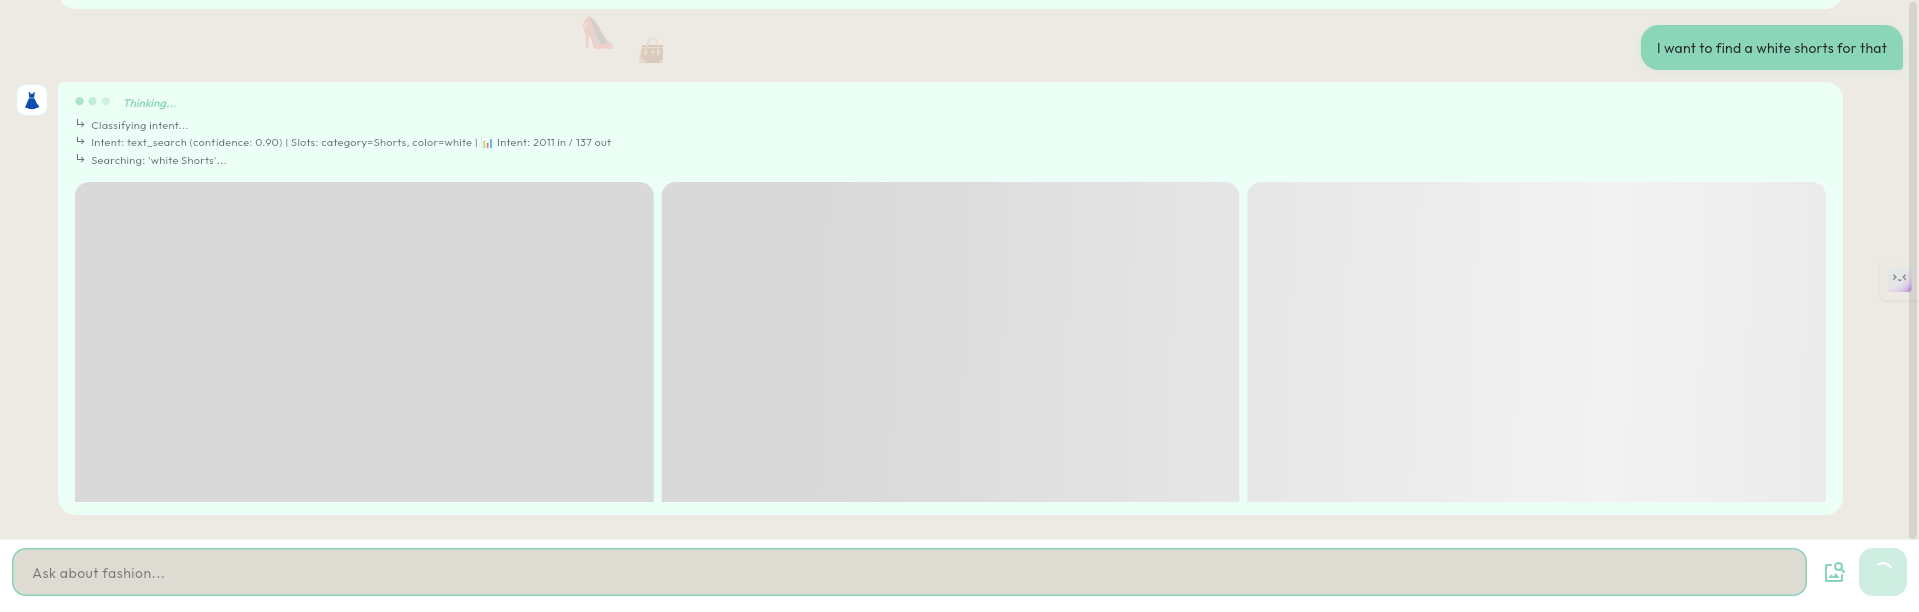
\includegraphics[width=0.85\textwidth]{screenshot_sse_streaming.png}
    \caption{Streamed thinking events visible to the user: the collapsible ``Thought for $t$ seconds'' header carries the input/output token counter populated from the \texttt{thinking\_end} event, and the synthesis tokens stream into the bubble live as \texttt{token} events arrive.}
    \label{fig:impl_sse_streaming}
\end{figure}


\section{System Integration and Deployment}
\label{sec:impl_deploy}

Section~\ref{sec:impl_deploy} describes how the components above are wired together into a single Compose stack, the bootstrap order enforced by the launcher, and the volume lifecycle that an operator must respect to avoid forcing the multi-hour re-ingestion pipeline. The ngrok agent service exposes the Flutter front-end on a stable public URL without opening any inbound port on the host.

\subsection{Compose Service Inventory}

Table~\ref{tab:impl_services} lists every Docker Compose service in the production profile, the image it builds from, the ports it binds, the volumes it attaches, and the upstream services it depends on. The optional \texttt{ngrok-fe} service exists but is gated behind the \texttt{ngrok} Compose profile and is therefore not part of the default-up topology.

\begin{table}[H]
\centering
\caption{Docker Compose services in the default profile.}
\label{tab:impl_services}
\small
\begin{tabular}{p{2.4cm} p{3.6cm} p{1.6cm} p{3.4cm} p{2.6cm}}
\toprule
\textbf{Service} & \textbf{Image} & \textbf{Port} & \textbf{Volumes} & \textbf{Depends-on} \\
\midrule
\texttt{postgres} & \texttt{postgres:16-alpine} & 5432 & \texttt{pgdata} (named) & --- \\
\texttt{qdrant} & \texttt{qdrant/qdrant:latest} & 6333 & \texttt{qdrant\_data} (named) & --- \\
\texttt{fashion-api} & built from \texttt{./Dockerfile} & 8000 & \texttt{./models}, \texttt{./images}, \texttt{\$\{DATASET\_IMAGES\_HOST\_PATH\}}, \texttt{./agent}, \texttt{./api} & \texttt{postgres} (healthy), \texttt{qdrant} (healthy) \\
\texttt{clothie-web} & built from \texttt{../clothie\_web} & 3000 & --- & \texttt{fashion-api} \\
\texttt{ngrok-fe} & \texttt{ngrok/ngrok:latest} & --- & --- & \texttt{clothie-web} \\
\bottomrule
\end{tabular}
\end{table}

The two database services have explicit healthchecks: Postgres uses \texttt{pg\_isready}, Qdrant uses a TCP probe on port 6333. The \texttt{fashion-api} \texttt{depends\_on} clause is gated on \texttt{condition: service\_healthy} for both, so the API container is not started until the data plane is ready to receive connections. Bind-mounts on \texttt{./agent} and \texttt{./api} keep the development feedback loop short --- a Python-only edit becomes effective on the next API restart without a rebuild.

\subsection{Container Topology}

Figure~\ref{fig:impl_topology} visualises the topology actually deployed, including the data-plane edges (\texttt{fashion-api} reads Postgres and Qdrant), the front-end edge (\texttt{clothie-web} consumes the API on port 3000), and the public-exposure path (\texttt{ngrok-fe} forwards a stable \texttt{*.ngrok-free.app} hostname onto \texttt{clothie-web:80}).

\begin{figure}[H]
\centering
\begin{tikzpicture}[
    node distance=10mm and 18mm,
    every node/.style={font=\footnotesize},
    service/.style={rectangle, draw, rounded corners=2pt, minimum width=2.6cm, minimum height=0.9cm, align=center, fill=blue!5},
    db/.style={service, fill=orange!10},
    front/.style={service, fill=green!10},
    edge/.style={service, fill=red!10},
    public/.style={rectangle, draw, rounded corners=8pt, minimum width=2.6cm, minimum height=1.0cm, align=center, fill=gray!10, dashed},
    arr/.style={->, thick},
    dep/.style={->, thick, dashed, gray}
]
    \node[db]   (pg)    {\texttt{postgres}\\\scriptsize:5432 \quad vol \texttt{pgdata}};
    \node[db, right=of pg] (qd) {\texttt{qdrant}\\\scriptsize:6333 \quad vol \texttt{qdrant\_data}};

    \node[service, below=of $(pg)!0.5!(qd)$] (api) {\texttt{fashion-api}\\\scriptsize:8000 \quad FastAPI + Gradio};

    \node[front, below=of api] (web) {\texttt{clothie-web}\\\scriptsize:3000 \quad Flutter + Nginx};

    \node[edge, right=of web] (ng) {\texttt{ngrok-fe}\\\scriptsize ngrok HTTP tunnel};

    \node[public, right=of ng] (net) {Public\\Internet};

    % Data plane
    \draw[arr] (api) -- node[left,scale=0.85] {SQL} (pg);
    \draw[arr] (api) -- node[right,scale=0.85] {HTTP} (qd);

    % Front-end plane
    \draw[arr] (web) -- node[right,scale=0.85] {\texttt{/api/*}} (api);

    % Public exposure: ngrok-fe -> clothie-web:80, and ngrok-fe -> public Internet
    \draw[arr] (ng) -- node[above,scale=0.85] {\texttt{:80}} (web);
    \draw[arr] (ng) -- node[above,scale=0.85] {\texttt{*.ngrok-free.app}} (net);


\end{tikzpicture}
\caption{Container topology of the Clothie deployment} 
\label{fig:impl_topology}
\end{figure}

\subsection{Bootstrap Sequence}

The repository ships a single launcher, \texttt{start.sh}, that an operator can run from the repository root. The launcher resolves the Docker binary on macOS (which adds Docker Desktop to the interactive PATH only), brings up the database services, waits for both healthchecks, builds and starts the application services, and tails the Cloudflared logs to extract the public URL. Algorithm~\ref{alg:bootstrap_clothie} formalises this sequence.

\begin{algorithm}[H]
\caption{BootstrapClothie}\label{alg:bootstrap_clothie}
\textit{Source: \texttt{start.sh}}
\begin{algorithmic}[1]
\Require Compose file \texttt{fashion\_agent/docker-compose.yml}, environment file \texttt{fashion\_agent/.env}
\Ensure A running stack with \texttt{fashion-api} reachable on port 8000 and a public Cloudflare URL printed
\State Resolve Docker binary on macOS by extending \texttt{PATH}
\State Verify that \texttt{docker} is on \texttt{PATH} and that the env file exists; abort with a diagnostic on failure
\State Run \texttt{dc up -d postgres qdrant} \Comment{databases first, isolated from API}
\For{$i \gets 1$ \textbf{to} $30$} \Comment{wait at most 60\,s}
    \State $h_{pg} \gets$ health of \texttt{postgres}; $h_{qd} \gets$ health of \texttt{qdrant}
    \If{$h_{pg} =$ \texttt{healthy} \textbf{and} $h_{qd} =$ \texttt{healthy}} \textbf{break} \EndIf
    \State sleep 2\,s
\EndFor
\State Run \texttt{dc up -d --build} \Comment{build / start \texttt{fashion-api}, \texttt{clothie-web}, \texttt{cloudflared-fe}}
\State $URL \gets \emptyset$
\For{$i \gets 1$ \textbf{to} $60$} \Comment{wait at most 60\,s for the tunnel}
    \State $URL \gets$ first match of \texttt{https://[a-z0-9-]+\.trycloudflare\.com} in \texttt{cloudflared-fe} logs
    \If{$URL \neq \emptyset$} \textbf{break} \EndIf
    \State sleep 1\,s
\EndFor
\If{$URL \neq \emptyset$} print the banner with $URL$, \texttt{http://localhost:3000}, \texttt{http://localhost:8000}
\Else{} print a fallback diagnostic pointing to \texttt{./start.sh --logs}
\EndIf
\end{algorithmic}
\end{algorithm}

The launcher accepts three subcommands beyond the default \texttt{up}: \texttt{--stop} runs \texttt{docker compose down} (preserving volumes), \texttt{--logs} tails the last 100 log lines per service, and \texttt{--status} prints \texttt{docker compose ps}. None of these subcommands ever invokes \texttt{down -v}; the destructive path is reserved for a deliberate, manual operator action.

\subsection{Environment Variables}

All credentials and behavioural switches are read from the \texttt{.env} file at Compose start; Table~\ref{tab:impl_env} lists the ones that affect runtime.

\begin{table}[H]
\centering
\caption{Environment variables consumed at runtime.}
\label{tab:impl_env}
\footnotesize
\setlength{\tabcolsep}{4pt}
\begin{tabular}{>{\raggedright\arraybackslash}p{4.6cm} >{\raggedright\arraybackslash}p{2.2cm} >{\raggedright\arraybackslash}p{7.2cm}}
\toprule
\textbf{Variable} & \textbf{Consumer} & \textbf{Default / Effect} \\
\midrule
\texttt{PG\_PASSWORD} & \texttt{postgres},\newline\texttt{fashion-api} & Required. \\
\texttt{PGHOST} / \texttt{PGPORT} /\newline\texttt{PGDATABASE} / \texttt{PGUSER} & \texttt{fashion-api} & \texttt{postgres}, \texttt{5432}, \texttt{fashion\_rag}, \texttt{fashion\_user}. \\
\texttt{QDRANT\_HOST} /\newline\texttt{QDRANT\_PORT} & \texttt{fashion-api} & \texttt{qdrant}, \texttt{6333}. \\
\texttt{QDRANT\_API\_KEY} & \texttt{fashion-api} & Empty (plain HTTP locally). \\
\texttt{GEMINI\_API\_KEY} & \texttt{fashion-api} & Required for any LLM call. \\
\texttt{ENABLE\_PATH2\_\allowbreak IMAGE\_SEARCH} & \texttt{fashion-api} & \texttt{false}; PATH 2 returns 503. \\
\texttt{PATH2\_MAX\_\allowbreak UPLOAD\_BYTES} /\newline\texttt{PATH2\_MAX\_TOP\_K} & \texttt{fashion-api} & 5\,MiB; 20. \\
\texttt{SEARCH\_CONFIDENCE\_\allowbreak THRESHOLD} & \texttt{fashion-api} & 0.75; slot-readiness gate (Algorithm~\ref{alg:slot_readiness}). \\
\texttt{DATASET\_IMAGES\_\allowbreak HOST\_PATH} & \texttt{fashion-api} & Mounted read-only at \texttt{/app/dataset\_images}; else \texttt{./images}. \\
\texttt{HF\_HOME} /\newline\texttt{TRANSFORMERS\_CACHE} & \texttt{fashion-api} & \texttt{/app/models} (encoder weight cache). \\
\texttt{ADMIN\_SECRET\_KEY} & \texttt{fashion-api} & Gates analytics endpoints (\texttt{X-Admin-Key}). \\
\texttt{NGROK\_AUTHTOKEN} & \texttt{ngrok-fe} & Required to start the agent. \\
\texttt{NGROK\_DOMAIN} & \texttt{ngrok-fe} & Reserved subdomain forwarded to \texttt{clothie-web:80}; falls back to the default hostname in the service definition. \\
\bottomrule
\end{tabular}
\end{table}

\subsection{Volume Lifecycle}

Two operations on the running stack look superficially similar but have very different consequences. \texttt{docker compose down} stops every container and removes the network, but leaves the named volumes \texttt{pgdata} and \texttt{qdrant\_data} intact; the next \texttt{up} resumes from the same state. \texttt{docker compose down -v} adds the volumes to the deletion set; the next \texttt{up} therefore starts from empty data directories, and the operator must either restore the two on-disk archives (Section~\ref{sec:impl_kb}) or re-run the multi-hour ingestion pipeline (\texttt{python -m pre\_processing.processing\_data} followed by \texttt{python -m indexing.build\_index}). The handover document explicitly forbids the destructive command for this reason.

\subsection{Public Exposure}

The production deployment exposes the Flutter front-end (port 3000 on the host, port 80 inside the Compose network) through the \texttt{ngrok-fe} service, which runs the official \texttt{ngrok/ngrok:latest} image with the command \texttt{http -{}-url=\$\{NGROK\_DOMAIN\} clothie-web:80}. The agent authenticates with \texttt{NGROK\_AUTHTOKEN} and binds a reserved subdomain (\texttt{*.ngrok-free.app}) so the public URL stays stable across restarts; this is the property an examiner relies on to revisit the live system without coordinating a fresh URL each session. No inbound port is opened on the host, no DNS record is provisioned, and all egress traffic flows through the long-lived ngrok agent connection. Operators read the live URL either from the \texttt{NGROK\_DOMAIN} they configured or from the ngrok agent's local status interface at \texttt{http://localhost:4040}; the launcher script's URL-discovery loop (Algorithm~\ref{alg:bootstrap_clothie}) is therefore vestigial under the ngrok path and is retained only for backward compatibility with the legacy Cloudflare Tunnel flow.